\documentclass[]{book}
\usepackage{lmodern}
\usepackage{amssymb,amsmath}
\usepackage{ifxetex,ifluatex}
\usepackage{fixltx2e} % provides \textsubscript
\ifnum 0\ifxetex 1\fi\ifluatex 1\fi=0 % if pdftex
  \usepackage[T1]{fontenc}
  \usepackage[utf8]{inputenc}
\else % if luatex or xelatex
  \ifxetex
    \usepackage{mathspec}
  \else
    \usepackage{fontspec}
  \fi
  \defaultfontfeatures{Ligatures=TeX,Scale=MatchLowercase}
\fi
% use upquote if available, for straight quotes in verbatim environments
\IfFileExists{upquote.sty}{\usepackage{upquote}}{}
% use microtype if available
\IfFileExists{microtype.sty}{%
\usepackage{microtype}
\UseMicrotypeSet[protrusion]{basicmath} % disable protrusion for tt fonts
}{}
\usepackage{hyperref}
\hypersetup{unicode=true,
            pdfborder={0 0 0},
            breaklinks=true}
\urlstyle{same}  % don't use monospace font for urls
\usepackage{natbib}
\bibliographystyle{apalike}
\usepackage{color}
\usepackage{fancyvrb}
\newcommand{\VerbBar}{|}
\newcommand{\VERB}{\Verb[commandchars=\\\{\}]}
\DefineVerbatimEnvironment{Highlighting}{Verbatim}{commandchars=\\\{\}}
% Add ',fontsize=\small' for more characters per line
\usepackage{framed}
\definecolor{shadecolor}{RGB}{248,248,248}
\newenvironment{Shaded}{\begin{snugshade}}{\end{snugshade}}
\newcommand{\AlertTok}[1]{\textcolor[rgb]{0.94,0.16,0.16}{#1}}
\newcommand{\AnnotationTok}[1]{\textcolor[rgb]{0.56,0.35,0.01}{\textbf{\textit{#1}}}}
\newcommand{\AttributeTok}[1]{\textcolor[rgb]{0.77,0.63,0.00}{#1}}
\newcommand{\BaseNTok}[1]{\textcolor[rgb]{0.00,0.00,0.81}{#1}}
\newcommand{\BuiltInTok}[1]{#1}
\newcommand{\CharTok}[1]{\textcolor[rgb]{0.31,0.60,0.02}{#1}}
\newcommand{\CommentTok}[1]{\textcolor[rgb]{0.56,0.35,0.01}{\textit{#1}}}
\newcommand{\CommentVarTok}[1]{\textcolor[rgb]{0.56,0.35,0.01}{\textbf{\textit{#1}}}}
\newcommand{\ConstantTok}[1]{\textcolor[rgb]{0.00,0.00,0.00}{#1}}
\newcommand{\ControlFlowTok}[1]{\textcolor[rgb]{0.13,0.29,0.53}{\textbf{#1}}}
\newcommand{\DataTypeTok}[1]{\textcolor[rgb]{0.13,0.29,0.53}{#1}}
\newcommand{\DecValTok}[1]{\textcolor[rgb]{0.00,0.00,0.81}{#1}}
\newcommand{\DocumentationTok}[1]{\textcolor[rgb]{0.56,0.35,0.01}{\textbf{\textit{#1}}}}
\newcommand{\ErrorTok}[1]{\textcolor[rgb]{0.64,0.00,0.00}{\textbf{#1}}}
\newcommand{\ExtensionTok}[1]{#1}
\newcommand{\FloatTok}[1]{\textcolor[rgb]{0.00,0.00,0.81}{#1}}
\newcommand{\FunctionTok}[1]{\textcolor[rgb]{0.00,0.00,0.00}{#1}}
\newcommand{\ImportTok}[1]{#1}
\newcommand{\InformationTok}[1]{\textcolor[rgb]{0.56,0.35,0.01}{\textbf{\textit{#1}}}}
\newcommand{\KeywordTok}[1]{\textcolor[rgb]{0.13,0.29,0.53}{\textbf{#1}}}
\newcommand{\NormalTok}[1]{#1}
\newcommand{\OperatorTok}[1]{\textcolor[rgb]{0.81,0.36,0.00}{\textbf{#1}}}
\newcommand{\OtherTok}[1]{\textcolor[rgb]{0.56,0.35,0.01}{#1}}
\newcommand{\PreprocessorTok}[1]{\textcolor[rgb]{0.56,0.35,0.01}{\textit{#1}}}
\newcommand{\RegionMarkerTok}[1]{#1}
\newcommand{\SpecialCharTok}[1]{\textcolor[rgb]{0.00,0.00,0.00}{#1}}
\newcommand{\SpecialStringTok}[1]{\textcolor[rgb]{0.31,0.60,0.02}{#1}}
\newcommand{\StringTok}[1]{\textcolor[rgb]{0.31,0.60,0.02}{#1}}
\newcommand{\VariableTok}[1]{\textcolor[rgb]{0.00,0.00,0.00}{#1}}
\newcommand{\VerbatimStringTok}[1]{\textcolor[rgb]{0.31,0.60,0.02}{#1}}
\newcommand{\WarningTok}[1]{\textcolor[rgb]{0.56,0.35,0.01}{\textbf{\textit{#1}}}}
\usepackage{longtable,booktabs}
\usepackage{graphicx,grffile}
\makeatletter
\def\maxwidth{\ifdim\Gin@nat@width>\linewidth\linewidth\else\Gin@nat@width\fi}
\def\maxheight{\ifdim\Gin@nat@height>\textheight\textheight\else\Gin@nat@height\fi}
\makeatother
% Scale images if necessary, so that they will not overflow the page
% margins by default, and it is still possible to overwrite the defaults
% using explicit options in \includegraphics[width, height, ...]{}
\setkeys{Gin}{width=\maxwidth,height=\maxheight,keepaspectratio}
\IfFileExists{parskip.sty}{%
\usepackage{parskip}
}{% else
\setlength{\parindent}{0pt}
\setlength{\parskip}{6pt plus 2pt minus 1pt}
}
\setlength{\emergencystretch}{3em}  % prevent overfull lines
\providecommand{\tightlist}{%
  \setlength{\itemsep}{0pt}\setlength{\parskip}{0pt}}
\setcounter{secnumdepth}{5}
% Redefines (sub)paragraphs to behave more like sections
\ifx\paragraph\undefined\else
\let\oldparagraph\paragraph
\renewcommand{\paragraph}[1]{\oldparagraph{#1}\mbox{}}
\fi
\ifx\subparagraph\undefined\else
\let\oldsubparagraph\subparagraph
\renewcommand{\subparagraph}[1]{\oldsubparagraph{#1}\mbox{}}
\fi

%%% Use protect on footnotes to avoid problems with footnotes in titles
\let\rmarkdownfootnote\footnote%
\def\footnote{\protect\rmarkdownfootnote}

%%% Change title format to be more compact
\usepackage{titling}

% Create subtitle command for use in maketitle
\providecommand{\subtitle}[1]{
  \posttitle{
    \begin{center}\large#1\end{center}
    }
}

\setlength{\droptitle}{-2em}

  \title{}
    \pretitle{\vspace{\droptitle}}
  \posttitle{}
    \author{}
    \preauthor{}\postauthor{}
    \date{}
    \predate{}\postdate{}
  
\usepackage{booktabs}

\begin{document}

{
\setcounter{tocdepth}{1}
\tableofcontents
}
\hypertarget{fitopatometruxeda}{%
\chapter*{Fitopatometría}\label{fitopatometruxeda}}
\addcontentsline{toc}{chapter}{Fitopatometría}

Rama de la fitopatología que se ocupa de la teoría y la práctica de la
evaluación cuantitativa de enfermedades (y/o patógenos).

\textbf{Nivel de planta individual}

\begin{itemize}
\tightlist
\item
  Severidad: medida de la cantidad de enfermedad por unidad de muestreo
  (planta, m² de cultivo, fruto, etc.) . En fitopatología es comúnmente
  definida como el área (volumen) de tejido enfermo dividido por el
  total del área (volumen) (x100 para obtener un valor en porcentaje)
\end{itemize}

\textbf{Nivel de parcela / lote}

\begin{itemize}
\item
  Incidencia: número de unidades muestreales (plantas) que están
  enfermas o infectadas por un agente patogénico. Expresado como un
  porcentaje (\%) o proporción (0-\textgreater{}1) del número total de
  unidades evaluadas.
\item
  Indice de severidad: Estimación de severidad usando una escala de
  severidad que comprende una serie de intervalos de rangos numéricos.
\end{itemize}

Por ej:

\begin{Shaded}
\begin{Highlighting}[]
\NormalTok{grado  rango de severidad}
\OperatorTok{-----}\StringTok{  }\OperatorTok{------------------}
\StringTok{    }\DecValTok{0}                   \DecValTok{0}
    \DecValTok{1}              \DecValTok{0}\OperatorTok{<=}\DecValTok{25}\NormalTok
    \DecValTok{3}             \DecValTok{50}\OperatorTok{<=}\DecValTok{75}\NormalTok
\end{Highlighting}
\end{Shaded}

La propuesta de \citet{madden2007study} (Cap. 2, pág. 20) es corregir
por el punto medio del rango de severidad:

\(IS(\%)=\frac {\sum frecuencia \: de \: grado\: \times\: punto \: medio \: del \: grado \:de\: escala} {total \: plantas \: evaluadas \times 100}\)

\textbf{Nivel de región}

\begin{itemize}
\tightlist
\item
  Prevalencia: número de unidades de muestreo geográficas (lotes,
  campos, municipios, estados, regiones, etc.) donde se detectó una
  enfermedad o un patógeno, dividido por el número total de unidades de
  muestreo geográficas evaluadas.
\end{itemize}

\hypertarget{manuxedcarbuxf3n---indice-de-severidad}{%
\chapter{Maní/carbón - Indice de
severidad}\label{manuxedcarbuxf3n---indice-de-severidad}}

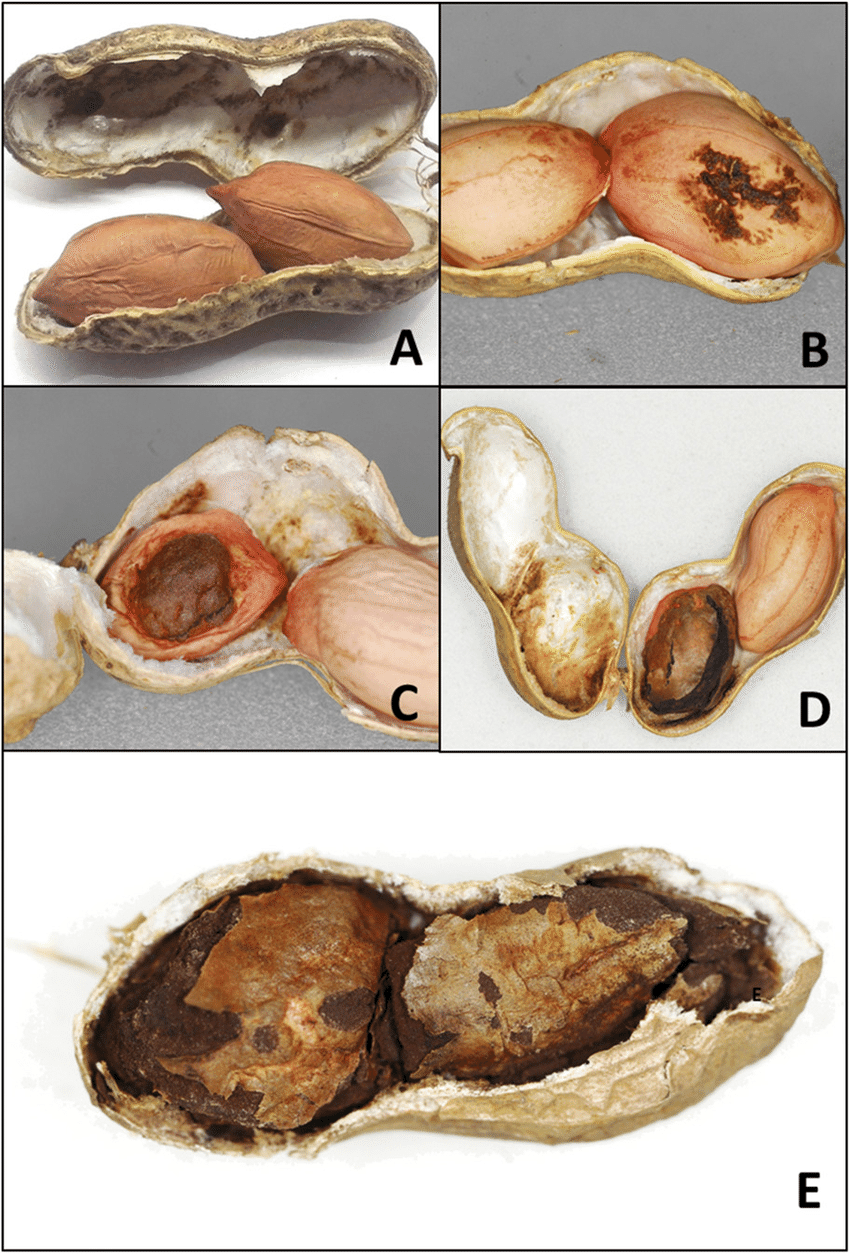
\includegraphics[width=2.08333in,height=\textheight]{fig/peanut_smut.png}

\begin{Shaded}
\begin{Highlighting}[]
\NormalTok{url_mani <-}\StringTok{ "https://docs.google.com/spreadsheets/d/1QJuQ2Zm26ufVYklB7vak6gQej3Xtyvbtj1yPKDlczD0/edit#gid=0"}

\NormalTok{mani <-}\StringTok{ }\NormalTok{gsheet}\OperatorTok{::}\KeywordTok{gsheet2tbl}\NormalTok{(url_mani)}

\NormalTok{url_mani <-}\StringTok{ }\NormalTok{url_mani }\OperatorTok\StringTok{ }
\StringTok{  }\KeywordTok{mutate_at}\NormalTok{(}\KeywordTok{vars}\NormalTok{(}\KeywordTok{c}\NormalTok{(}\StringTok{"trt"}\NormalTok{, }\StringTok{"sprays"}\NormalTok{, }\StringTok{"bk"}\NormalTok{)),}\KeywordTok{funs}\NormalTok{(factor)) }

\NormalTok{mani}
\end{Highlighting}
\end{Shaded}

Exploramos cuántas plantas (sub-muestra) fueron evaluadas por parcela:

\begin{Shaded}
\begin{Highlighting}[]
\NormalTok{mani }\OperatorTok
\StringTok{  }\KeywordTok{group_by}\NormalTok{(trt, sprays, bk)}\OperatorTok
\StringTok{  }\KeywordTok{summarise}\NormalTok{(}\DataTypeTok{n=}\KeywordTok{n}\NormalTok{()) }\CommentTok{#%>% knitr::kable()}
\end{Highlighting}
\end{Shaded}

Calculamos la incidencia por parcela y agregamos una columna para
identificar a la planta como sub-muestra dentro de cada parcela:

\begin{Shaded}
\begin{Highlighting}[]
\NormalTok{mani1 <-}\StringTok{ }\NormalTok{mani }\OperatorTok\StringTok{ }
\StringTok{  }\KeywordTok{mutate}\NormalTok{(}
    \DataTypeTok{trt =} \KeywordTok{relevel}\NormalTok{(trt, }\DataTypeTok{ref=}\StringTok{"check"}\NormalTok{),}
    \DataTypeTok{dis_pod =} \KeywordTok{rowSums}\NormalTok{(}\KeywordTok{select}\NormalTok{(., }\KeywordTok{matches}\NormalTok{(}\StringTok{'x1|x2|x3|x4'}\NormalTok{))),}
    \DataTypeTok{inc =}\NormalTok{ dis_pod}\OperatorTok{/}\NormalTok{n_pods,}
    \DataTypeTok{x0_p =} \KeywordTok{rowSums}\NormalTok{(}\KeywordTok{select}\NormalTok{(., }\KeywordTok{matches}\NormalTok{(}\StringTok{'x0'}\NormalTok{)))}\OperatorTok{/}\NormalTok{n_pods,}
    \DataTypeTok{x3.4 =} \KeywordTok{rowSums}\NormalTok{(}\KeywordTok{select}\NormalTok{(., }\KeywordTok{matches}\NormalTok{(}\StringTok{'x3|x4'}\NormalTok{))), }
    \DataTypeTok{sev0_1 =}\NormalTok{ (}\DecValTok{0}\OperatorTok{*}\NormalTok{x0 }\OperatorTok{+}\StringTok{ }\FloatTok{0.01}\OperatorTok{*}\NormalTok{x1 }\FloatTok{+0.1}\OperatorTok{*}\NormalTok{x2 }\OperatorTok{+}\StringTok{ }\FloatTok{0.7}\OperatorTok{*}\NormalTok{x3 }\OperatorTok{+}\StringTok{ }\DecValTok{1}\OperatorTok{*}\NormalTok{x4)}\OperatorTok{/}\StringTok{ }\NormalTok{n_pods) }\OperatorTok\StringTok{ }
\StringTok{  }\KeywordTok{group_by}\NormalTok{(sprays, trt, bk) }\OperatorTok
\StringTok{  }\KeywordTok{mutate}\NormalTok{(}\DataTypeTok{sample =} \KeywordTok{row_number}\NormalTok{()) }\OperatorTok\StringTok{ }
\StringTok{  }
\StringTok{  }\CommentTok{# filter(sprays!=1, }
\StringTok{  }\CommentTok{#        trt!="Epoxiconazole") %>%}
\StringTok{  }\NormalTok{ungroup }

\NormalTok{mani1}
\end{Highlighting}
\end{Shaded}

\hypertarget{colzaphoma---uxe1rea-abajo-la-curva}{%
\chapter{Colza/phoma - Área abajo la
curva}\label{colzaphoma---uxe1rea-abajo-la-curva}}

Calcularemos un valor de AUC por parcela con auxilio de las funciones
\texttt{group\_by} y \texttt{summarize}

\begin{Shaded}
\begin{Highlighting}[]
\CommentTok{# if(require(MESS)) \{install.packages("MESS")\}}
\NormalTok{can_long }\OperatorTok
\StringTok{  }\KeywordTok{group_by}\NormalTok{(trt, bk) }\OperatorTok
\StringTok{  }\KeywordTok{summarize}\NormalTok{(}\DataTypeTok{AUC =}\NormalTok{ MESS}\OperatorTok{::}\KeywordTok{auc}\NormalTok{(inc, tt))}
\end{Highlighting}
\end{Shaded}

\hypertarget{olivoxylella---prevalencia}{%
\chapter{Olivo/xylella - prevalencia}\label{olivoxylella---prevalencia}}

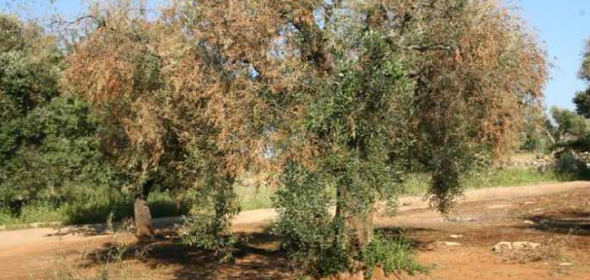
\includegraphics{fig/xylella.jpg}

Chequeamos cuántos árboles fueron evaluados en cada año/región/lote:

\begin{Shaded}
\begin{Highlighting}[]
\KeywordTok{ftable}\NormalTok{(}\KeywordTok{xtabs}\NormalTok{(}\OperatorTok{~}\NormalTok{year}\OperatorTok{+}\NormalTok{loc}\OperatorTok{+}\NormalTok{farm, oli_long))}
\end{Highlighting}
\end{Shaded}

Imprimimos los 30 árboles de un mismo lote

\begin{Shaded}
\begin{Highlighting}[]
\NormalTok{oli_long }\OperatorTok\StringTok{ }
\StringTok{  }\KeywordTok{arrange}\NormalTok{(loc, year) }\OperatorTok\StringTok{ }
\StringTok{  }\KeywordTok{print}\NormalTok{(}\DataTypeTok{n=}\DecValTok{30}\NormalTok{)}
\end{Highlighting}
\end{Shaded}

Incidencia (nivel lote - evolución interanual)

\begin{Shaded}
\begin{Highlighting}[]
\NormalTok{dat_inc <-}\StringTok{ }\NormalTok{oli_long }\OperatorTok
\StringTok{  }\KeywordTok{group_by}\NormalTok{(year, loc, farm) }\OperatorTok
\StringTok{  }\KeywordTok{summarise}\NormalTok{(}\DataTypeTok{inc =} \KeywordTok{mean}\NormalTok{(sev}\OperatorTok{>}\DecValTok{0}\NormalTok{, }\DataTypeTok{na.rm=}\OtherTok{TRUE}\NormalTok{)}\OperatorTok{*}\DecValTok{100}\NormalTok{) }\OperatorTok\StringTok{ }
\StringTok{  }\NormalTok{ungroup }\OperatorTok\StringTok{ }
\StringTok{  }\KeywordTok{arrange}\NormalTok{(loc, year)}
\NormalTok{dat_inc}
\end{Highlighting}
\end{Shaded}

\begin{Shaded}
\begin{Highlighting}[]
\KeywordTok{ggplot}\NormalTok{(dat_inc, }\KeywordTok{aes}\NormalTok{(}\DataTypeTok{x=}\KeywordTok{factor}\NormalTok{(year), }\DataTypeTok{y=}\NormalTok{inc, }\DataTypeTok{color=}\KeywordTok{factor}\NormalTok{(farm))) }\OperatorTok{+}
\StringTok{  }\KeywordTok{geom_point}\NormalTok{() }\OperatorTok{+}
\StringTok{  }\KeywordTok{geom_line}\NormalTok{(}\KeywordTok{aes}\NormalTok{(}\DataTypeTok{group=}\NormalTok{farm)) }\OperatorTok{+}
\StringTok{  }\KeywordTok{facet_grid}\NormalTok{(. }\OperatorTok{~}\StringTok{ }\NormalTok{loc)}
\end{Highlighting}
\end{Shaded}

Prevalencia (nivel región - evolución interanual)

\begin{Shaded}
\begin{Highlighting}[]
\NormalTok{dat_prev  <-}\StringTok{ }\NormalTok{dat_inc }\OperatorTok
\StringTok{  }\KeywordTok{group_by}\NormalTok{(year, loc) }\OperatorTok
\StringTok{  }\KeywordTok{summarise}\NormalTok{(}\DataTypeTok{prev =} \KeywordTok{trunc}\NormalTok{(}\KeywordTok{mean}\NormalTok{(inc}\OperatorTok{>}\DecValTok{0}\NormalTok{, }\DataTypeTok{na.rm=}\OtherTok{TRUE}\NormalTok{)}\OperatorTok{*}\DecValTok{100}\NormalTok{)) }\OperatorTok\StringTok{ }
\StringTok{  }\NormalTok{ungroup }\OperatorTok\StringTok{ }
\StringTok{  }\KeywordTok{arrange}\NormalTok{(loc,year)}
\NormalTok{dat_prev}
\end{Highlighting}
\end{Shaded}

\begin{Shaded}
\begin{Highlighting}[]
\KeywordTok{ggplot}\NormalTok{(dat_prev, }\KeywordTok{aes}\NormalTok{(}\DataTypeTok{x=}\KeywordTok{factor}\NormalTok{(year), }\DataTypeTok{y=}\NormalTok{prev, }\DataTypeTok{color=}\KeywordTok{factor}\NormalTok{(loc))) }\OperatorTok{+}
\StringTok{  }\KeywordTok{geom_point}\NormalTok{() }\OperatorTok{+}
\StringTok{  }\KeywordTok{geom_line}\NormalTok{(}\KeywordTok{aes}\NormalTok{(}\DataTypeTok{group=}\NormalTok{loc))}
\end{Highlighting}
\end{Shaded}

\begin{Shaded}
\begin{Highlighting}[]
\NormalTok{pacman}\OperatorTok{::}\KeywordTok{p_load}\NormalTok{(tidyverse, tidyselect)}
\end{Highlighting}
\end{Shaded}

\hypertarget{trigoenfermedades-foliares---retenciuxf3n-foliar}{%
\chapter{Trigo/enfermedades foliares - retención
foliar}\label{trigoenfermedades-foliares---retenciuxf3n-foliar}}

\begin{Shaded}
\begin{Highlighting}[]
\NormalTok{url_trigo <-}\StringTok{ "https://docs.google.com/spreadsheets/d/1QJuQ2Zm26ufVYklB7vak6gQej3Xtyvbtj1yPKDlczD0/edit#gid=407239570"}
\CommentTok{# browseURL(url)}
\NormalTok{trigo <-}\StringTok{ }\NormalTok{gsheet}\OperatorTok{::}\KeywordTok{gsheet2tbl}\NormalTok{(url_trigo)}
\end{Highlighting}
\end{Shaded}

\begin{itemize}
\item
  Manipulación
\item
  Clasificar variables
\end{itemize}

\begin{Shaded}
\begin{Highlighting}[]
\NormalTok{trigo }\OperatorTok
\StringTok{  }\KeywordTok{mutate_at}\NormalTok{(}\KeywordTok{vars}\NormalTok{(}\KeywordTok{contains}\NormalTok{(}\StringTok{'.'}\NormalTok{)), }\KeywordTok{funs}\NormalTok{(factor)) }\OperatorTok
\StringTok{  }\KeywordTok{mutate_at}\NormalTok{(}\KeywordTok{vars}\NormalTok{(}\KeywordTok{contains}\NormalTok{(}\StringTok{'_'}\NormalTok{)), }\KeywordTok{funs}\NormalTok{(}\KeywordTok{as.numeric}\NormalTok{(}\KeywordTok{as.character}\NormalTok{(.))))}
\end{Highlighting}
\end{Shaded}

\begin{itemize}
\item
  dejar las observaciones crudas a nivel de submuestra/órgano en cada
  línea
\item
  eliminar submuestras no evaluadas
\item
  reemplazar NA's por 0
\item
  reorganizar dataset: wide -\textgreater{} long
\end{itemize}

\begin{Shaded}
\begin{Highlighting}[]
\NormalTok{trigo }\OperatorTok\StringTok{ }
\StringTok{  }\KeywordTok{pivot_longer}\NormalTok{(}\KeywordTok{contains}\NormalTok{(}\StringTok{"_"}\NormalTok{), }
               \DataTypeTok{names_to =} \StringTok{"org.var"}\NormalTok{, }\DataTypeTok{values_to =} \StringTok{"y"}\NormalTok{) }\OperatorTok\StringTok{ }
\StringTok{  }\KeywordTok{separate}\NormalTok{(org.var, }\KeywordTok{c}\NormalTok{(}\StringTok{"org."}\NormalTok{, }\StringTok{"var."}\NormalTok{)) }\OperatorTok\StringTok{ }
\StringTok{  }\KeywordTok{mutate_at}\NormalTok{(}\KeywordTok{vars}\NormalTok{(}\KeywordTok{contains}\NormalTok{(}\StringTok{'.'}\NormalTok{)), }\KeywordTok{funs}\NormalTok{(factor)) }\OperatorTok\StringTok{  }
\StringTok{  }\KeywordTok{pivot_wider}\NormalTok{(}\DataTypeTok{names_from =}\NormalTok{ var., }\DataTypeTok{values_from =}\NormalTok{ y) }\OperatorTok\StringTok{ }
\StringTok{  }\KeywordTok{filter}\NormalTok{(stringr}\OperatorTok{::}\KeywordTok{str_detect}\NormalTok{(org., }\StringTok{"b"}\NormalTok{)) }\OperatorTok\StringTok{ }\CommentTok{# elimina tallo }
\StringTok{  }\KeywordTok{filter}\NormalTok{(}\OperatorTok{!}\NormalTok{(}\KeywordTok{is.na}\NormalTok{(af))) }\OperatorTok\StringTok{  }\CommentTok{# elimina hojas perdidas}
\StringTok{  }\KeywordTok{mutate_if}\NormalTok{(is.numeric, }\OperatorTok{~}\KeywordTok{replace}\NormalTok{(., }\KeywordTok{is.na}\NormalTok{(.), }\DecValTok{0}\NormalTok{)) }\OperatorTok\StringTok{ }\CommentTok{# rellena con 0}
\StringTok{  }\KeywordTok{select}\NormalTok{(}\OperatorTok{-}\NormalTok{ry) ->}\StringTok{ }\NormalTok{datf }
\end{Highlighting}
\end{Shaded}

\begin{itemize}
\tightlist
\item
  Cálculos
\item
  resumir af media a nivel de parcela/órgano
\end{itemize}

\begin{Shaded}
\begin{Highlighting}[]
\NormalTok{datf }\OperatorTok\StringTok{ }
\StringTok{  }\KeywordTok{group_by}\NormalTok{(par., org.) }\OperatorTok\StringTok{ }
\StringTok{    }\KeywordTok{mutate}\NormalTok{(}
    \DataTypeTok{af_p =} \KeywordTok{case_when}\NormalTok{(}
\NormalTok{    af }\OperatorTok{==}\StringTok{ }\DecValTok{0} \OperatorTok{~}\StringTok{ }\NormalTok{(}\DecValTok{25}\OperatorTok{+}\DecValTok{0}\NormalTok{)}\OperatorTok{/}\DecValTok{2}\NormalTok{,}
\NormalTok{    af }\OperatorTok{==}\StringTok{ }\DecValTok{1} \OperatorTok{~}\StringTok{ }\NormalTok{(}\DecValTok{50}\OperatorTok{+}\DecValTok{25}\NormalTok{)}\OperatorTok{/}\DecValTok{2}\NormalTok{,}
\NormalTok{    af }\OperatorTok{==}\StringTok{ }\DecValTok{2} \OperatorTok{~}\StringTok{ }\NormalTok{(}\DecValTok{75}\OperatorTok{+}\DecValTok{50}\NormalTok{)}\OperatorTok{/}\DecValTok{2}\NormalTok{,}
\NormalTok{    af }\OperatorTok{==}\StringTok{ }\DecValTok{3} \OperatorTok{~}\StringTok{ }\NormalTok{(}\DecValTok{100}\OperatorTok{+}\DecValTok{75}\NormalTok{)}\OperatorTok{/}\DecValTok{2}\NormalTok{, }
    \DataTypeTok{af =} \OtherTok{TRUE} \OperatorTok{~}\StringTok{ }\NormalTok{af)) }\OperatorTok
\StringTok{  }\KeywordTok{summarise}\NormalTok{(}\DataTypeTok{trt. =} \KeywordTok{first}\NormalTok{(trt.),}
            \DataTypeTok{bq. =} \KeywordTok{first}\NormalTok{(bq.), }
            \DataTypeTok{af_p =} \KeywordTok{mean}\NormalTok{(af_p, }\DataTypeTok{na.rm =} \OtherTok{TRUE}\NormalTok{)) }\OperatorTok\StringTok{ }
\StringTok{  }\KeywordTok{select}\NormalTok{(trt., bq., }\KeywordTok{everything}\NormalTok{()) ->}\StringTok{ }\NormalTok{af_dat}
\end{Highlighting}
\end{Shaded}

\begin{itemize}
\tightlist
\item
  Incidencia media a nivel de parcela/órgano de cada enfermedad
\end{itemize}

\begin{Shaded}
\begin{Highlighting}[]
\NormalTok{datf }\OperatorTok\StringTok{ }\KeywordTok{select}\NormalTok{(}\OperatorTok{-}\NormalTok{af) }\OperatorTok\StringTok{ }
\StringTok{  }\KeywordTok{group_by}\NormalTok{(par., org.) }\OperatorTok\StringTok{ }
\StringTok{  }\KeywordTok{summarise_if}\NormalTok{(is.numeric, }
               \KeywordTok{funs}\NormalTok{(}\KeywordTok{round}\NormalTok{(}\KeywordTok{mean}\NormalTok{(.}\OperatorTok{>}\DecValTok{0}\NormalTok{, }\DataTypeTok{na.rm =} \OtherTok{TRUE}\NormalTok{)}\OperatorTok{*}\DecValTok{100}\NormalTok{))) ->}\StringTok{ }\NormalTok{inc_dat}
\end{Highlighting}
\end{Shaded}

\begin{itemize}
\tightlist
\item
  Severidad media a nivel de parcela/órgano de cada enfermedad
\end{itemize}

\begin{Shaded}
\begin{Highlighting}[]
\NormalTok{datf }\OperatorTok\StringTok{ }\KeywordTok{select}\NormalTok{(}\OperatorTok{-}\NormalTok{af) }\OperatorTok
\StringTok{  }\KeywordTok{group_by}\NormalTok{(par., org.) }\OperatorTok\StringTok{ }
\StringTok{  }\KeywordTok{summarise_if}\NormalTok{(is.numeric, }
               \KeywordTok{funs}\NormalTok{(}\KeywordTok{round}\NormalTok{(}\KeywordTok{mean}\NormalTok{(., }\DataTypeTok{na.rm =} \OtherTok{TRUE}\NormalTok{)))) ->}\StringTok{ }\NormalTok{sev_dat}
\end{Highlighting}
\end{Shaded}

\begin{itemize}
\tightlist
\item
  Unificar tablas
\end{itemize}

\begin{Shaded}
\begin{Highlighting}[]
\NormalTok{af_dat }\OperatorTok\StringTok{      }\CommentTok{# tabla con variables experimentales y af }
\StringTok{  }\KeywordTok{left_join}\NormalTok{(}\DataTypeTok{by =} \KeywordTok{c}\NormalTok{(}\StringTok{"par."}\NormalTok{, }\StringTok{"org."}\NormalTok{), }
\NormalTok{            (inc_dat }\OperatorTok\StringTok{   }\CommentTok{# tabla con variables de enfermedad }
\StringTok{              }\KeywordTok{left_join}\NormalTok{(sev_dat, }
                        \DataTypeTok{by =} \KeywordTok{c}\NormalTok{(}\StringTok{"par."}\NormalTok{, }\StringTok{"org."}\NormalTok{), }
                        \DataTypeTok{suffix=}\KeywordTok{c}\NormalTok{(}\StringTok{'_inc'}\NormalTok{, }\StringTok{'_sev'}\NormalTok{)))}
\NormalTok{  ) ->}\StringTok{ }\NormalTok{dat_foliar }
\end{Highlighting}
\end{Shaded}

\begin{itemize}
\item
  Métricas varias
\item
  Retencion foliar
\end{itemize}

\begin{Shaded}
\begin{Highlighting}[]
\NormalTok{hj_}\DecValTok{01}\NormalTok{ =}\StringTok{ }\KeywordTok{c}\NormalTok{(}\StringTok{"b0"}\NormalTok{,}\StringTok{"b1"}\NormalTok{)}
\NormalTok{hj_}\DecValTok{012}\NormalTok{=}\StringTok{ }\KeywordTok{c}\NormalTok{(}\StringTok{"b0"}\NormalTok{,}\StringTok{"b1"}\NormalTok{,}\StringTok{"b2"}\NormalTok{)}
\NormalTok{hj_}\DecValTok{23}\NormalTok{ =}\StringTok{ }\KeywordTok{c}\NormalTok{(}\StringTok{"b2"}\NormalTok{,}\StringTok{"b3"}\NormalTok{)}

\NormalTok{datf }\OperatorTok\StringTok{ }\CommentTok{#}
\StringTok{  }\KeywordTok{filter}\NormalTok{(org. }\OperatorTok\StringTok{ }\NormalTok{hj_}\DecValTok{012}\NormalTok{) }\OperatorTok\StringTok{ }
\StringTok{  }\KeywordTok{group_by}\NormalTok{(par.) }\OperatorTok\StringTok{ }
\StringTok{  }\KeywordTok{summarise}\NormalTok{(}\DataTypeTok{trt. =} \KeywordTok{first}\NormalTok{(trt.),}
            \DataTypeTok{bq. =} \KeywordTok{first}\NormalTok{(bq.),}
            \DataTypeTok{n =} \KeywordTok{n}\NormalTok{(),}
            \DataTypeTok{af_v =} \KeywordTok{mean}\NormalTok{(af}\OperatorTok{>}\DecValTok{1}\NormalTok{, }\DataTypeTok{na.rm =} \OtherTok{TRUE}\NormalTok{)) }\OperatorTok\StringTok{ }
\StringTok{    }\KeywordTok{ungroup}\NormalTok{() }\OperatorTok
\StringTok{  }\KeywordTok{mutate}\NormalTok{(}
    \DataTypeTok{order =} \KeywordTok{as.integer}\NormalTok{(}\KeywordTok{as.character}\NormalTok{(trt.)),}
    \DataTypeTok{trt1 =} \KeywordTok{fct_reorder}\NormalTok{(trt., order)}
\NormalTok{  ) }\OperatorTok\StringTok{ }
\StringTok{  }\KeywordTok{ggplot}\NormalTok{(}\KeywordTok{aes}\NormalTok{(}\DataTypeTok{x=}\NormalTok{trt1, }\DataTypeTok{y =}\NormalTok{af_v))}\OperatorTok{+}
\StringTok{  }\KeywordTok{stat_summary}\NormalTok{(}\DataTypeTok{fun.data =} \StringTok{"mean_cl_boot"}\NormalTok{, }\DataTypeTok{size =} \FloatTok{0.2}\NormalTok{)}\OperatorTok{+}
\StringTok{  }\KeywordTok{geom_jitter}\NormalTok{(}\KeywordTok{aes}\NormalTok{(}\DataTypeTok{col=}\NormalTok{bq.), }\DataTypeTok{width =} \FloatTok{0.2}\NormalTok{)}\OperatorTok{+}
\StringTok{  }\KeywordTok{labs}\NormalTok{(}\DataTypeTok{x=}\StringTok{""}\NormalTok{, }
       \DataTypeTok{y=}\StringTok{"% de hojas HB, HB-1 y HB-2 fotosint. activas}\CharTok{\textbackslash{}n}\StringTok{(>50% verdes)"}\NormalTok{)}\OperatorTok{+}
\StringTok{  }\KeywordTok{theme_bw}\NormalTok{()}
\end{Highlighting}
\end{Shaded}

\begin{Shaded}
\begin{Highlighting}[]
\NormalTok{dat_foliar }\OperatorTok\StringTok{ }\CommentTok{#}
\StringTok{  }\KeywordTok{filter}\NormalTok{(org. }\OperatorTok\StringTok{ }\NormalTok{hj_}\DecValTok{012}\NormalTok{) }\OperatorTok\StringTok{ }
\StringTok{  }\KeywordTok{group_by}\NormalTok{(par.) }\OperatorTok\StringTok{ }
\StringTok{  }\KeywordTok{summarise}\NormalTok{(}\DataTypeTok{trt. =} \KeywordTok{first}\NormalTok{(trt.),}
            \DataTypeTok{bq. =} \KeywordTok{first}\NormalTok{(bq.),}
            \DataTypeTok{n =} \KeywordTok{n}\NormalTok{(),}
            \DataTypeTok{ma_inc =} \KeywordTok{mean}\NormalTok{(ma_inc, }\DataTypeTok{na.rm =} \OtherTok{TRUE}\NormalTok{)) }\OperatorTok\StringTok{ }
\StringTok{  }\KeywordTok{ungroup}\NormalTok{() }\OperatorTok
\StringTok{  }\KeywordTok{mutate}\NormalTok{(}
    \DataTypeTok{order =} \KeywordTok{as.integer}\NormalTok{(}\KeywordTok{as.character}\NormalTok{(trt.)),}
    \DataTypeTok{trt1 =} \KeywordTok{fct_reorder}\NormalTok{(trt., order)}
\NormalTok{  ) }\OperatorTok\StringTok{ }
\StringTok{  }\KeywordTok{ggplot}\NormalTok{(}\KeywordTok{aes}\NormalTok{(}\DataTypeTok{x=}\NormalTok{trt1, }\DataTypeTok{y =}\NormalTok{ma_inc))}\OperatorTok{+}
\StringTok{  }\KeywordTok{stat_summary}\NormalTok{(}\DataTypeTok{fun.data =} \StringTok{"mean_cl_boot"}\NormalTok{, }\DataTypeTok{size =} \FloatTok{0.2}\NormalTok{)}\OperatorTok{+}
\StringTok{  }\KeywordTok{geom_jitter}\NormalTok{(}\KeywordTok{aes}\NormalTok{(}\DataTypeTok{col=}\NormalTok{bq.), }\DataTypeTok{width =} \FloatTok{0.2}\NormalTok{)}\OperatorTok{+}
\StringTok{  }\KeywordTok{labs}\NormalTok{(}\DataTypeTok{x=}\StringTok{""}\NormalTok{, }
       \DataTypeTok{y=}\StringTok{"Incidencia de mancha amarilla en HB y Hb-1"}\NormalTok{)}\OperatorTok{+}
\StringTok{  }\KeywordTok{theme_bw}\NormalTok{()}
\end{Highlighting}
\end{Shaded}

\begin{Shaded}
\begin{Highlighting}[]
\NormalTok{hojas <-}\StringTok{ }\KeywordTok{c}\NormalTok{(}
  \StringTok{`}\DataTypeTok{b0}\StringTok{`}\NormalTok{ =}\StringTok{ "Hj B"}\NormalTok{,}
  \StringTok{`}\DataTypeTok{b1}\StringTok{`}\NormalTok{ =}\StringTok{ "Hj B-1"}\NormalTok{,}
  \StringTok{`}\DataTypeTok{b2}\StringTok{`}\NormalTok{ =}\StringTok{ "Hj B-2"}\NormalTok{,}
  \StringTok{`}\DataTypeTok{b3}\StringTok{`}\NormalTok{ =}\StringTok{ "Hj B-3"}
\NormalTok{)}

\NormalTok{dat_foliar }\OperatorTok\StringTok{ }
\StringTok{  }\KeywordTok{ungroup}\NormalTok{() }\OperatorTok
\StringTok{  }\KeywordTok{mutate}\NormalTok{(}
    \DataTypeTok{order =} \KeywordTok{as.integer}\NormalTok{(}\KeywordTok{as.character}\NormalTok{(trt.)),}
    \DataTypeTok{trt1 =} \KeywordTok{fct_reorder}\NormalTok{(trt., order)}
\NormalTok{  ) }\OperatorTok\StringTok{ }
\StringTok{  }\KeywordTok{ggplot}\NormalTok{(}\KeywordTok{aes}\NormalTok{(}\DataTypeTok{x=}\NormalTok{trt1, }\DataTypeTok{y=}\NormalTok{af_p))}\OperatorTok{+}
\StringTok{  }\KeywordTok{geom_point}\NormalTok{(}\DataTypeTok{size =} \FloatTok{0.1}\NormalTok{) }\OperatorTok{+}\StringTok{ }
\StringTok{  }\KeywordTok{stat_summary}\NormalTok{(}\DataTypeTok{fun.data =} \StringTok{"mean_cl_boot"}\NormalTok{, }\DataTypeTok{colour =} \StringTok{"red"}\NormalTok{, }\DataTypeTok{size =} \FloatTok{0.2}\NormalTok{)}\OperatorTok{+}
\StringTok{  }\KeywordTok{facet_grid}\NormalTok{(org.}\OperatorTok{~}\NormalTok{.,}
             \DataTypeTok{labeller =} \KeywordTok{as_labeller}\NormalTok{(hojas))}\OperatorTok{+}
\StringTok{  }\KeywordTok{labs}\NormalTok{(}\DataTypeTok{y=}\StringTok{"% de área verde"}\NormalTok{, }\DataTypeTok{x=}\StringTok{"Tratamientos"}\NormalTok{)}\OperatorTok{+}\StringTok{  }
\StringTok{  }\KeywordTok{theme_bw}\NormalTok{()}
\end{Highlighting}
\end{Shaded}

\bibliography{book.bib,packages.bib}


\end{document}
